\section{Manuale Utente}
Grazie alle scelte tecnologiche con cui sono stati implementati i diversi componenti, il prodotto software può essere utilizzato ovunque e sulla maggior parte dei sistemi operativi, sia desktop (Windows, MacOs, Linux), sia mobile (Android o iOs).\todo{Davide chiede: "Si scrive così iOs?"}
L'applicativo si compone di quattro macro componenti:
\begin{itemize}
	\item \textbf{Web Server Spring}: questa componente è in esecuzione su una istanza di Azure Sping Clound e di conseguenza è sempre accessibile dall'applicazione client;
	\item \textbf{Database MySql}: anch'esso in esecuzione su una istanza di Azure MySql;
	\item \textbf{Data Collector e Data Analyzer}: queste due applicazioni sono in esecuzione su un Rapsberry Pi 4;
	\item \textbf{Applicazione Client}: grazie al framework Qt, tale applicazione può essere compilata ed essere eseguita su una gran parte dei sistemi operativi. Infatti, l'unica cosa che deve fare l'utente è installare l'APK sul proprio telefono, oppure installare l'applicazione sul proprio computer. 
\end{itemize}

In questo modo, l'utente può accedere ed utilizzate l'applicazione ed i servizi offerti in qualunque momento. 
\\
\\
In figura \ref{fig:qtApp}a viene mostrata la schermata di login dell'applicazione. Per accedere alle funzionalità, l'utente deve inserire lo username e la password che gli sono stati fornite dal coordinatore. 
Dopo aver inserito le credenziali, l'utente accede alla dashboard (figura \ref{fig:qtApp}b) in cui è possibile osservare alcune informazioni sul proprio account ed una mappa che mostra la posizione dell'area di appartenenza.
Nel menù laterale è possibile scegliere quali funzionalità utilizzare (figura \ref{fig:qtApp}c): si possono visualizzare informazioni meteorologiche (figura \ref{fig:qtApp}e), allarmi (figura \ref{fig:qtApp}d) o informazioni sul proprio account e sul proprio team, compresi alcuni dati sui membri del team (figura \ref{fig:qtApp}f).

Il coordinatore potrà invece scegliere dei servizi diversi da quelli di un utente normale (figura \ref{fig:qtApp2}a). Infatti, tale figura ha il compito di inserire nuovi volontari inserendone i dati (figura \ref{fig:qtApp2}b), creare nuove squadre e cancellare degli utenti (figura \ref{fig:qtApp2}c).
\todo{Da rileggere}

\begin{figure}[h!]
	\centering
	\subfloat[\centering Schermata di Login.]{{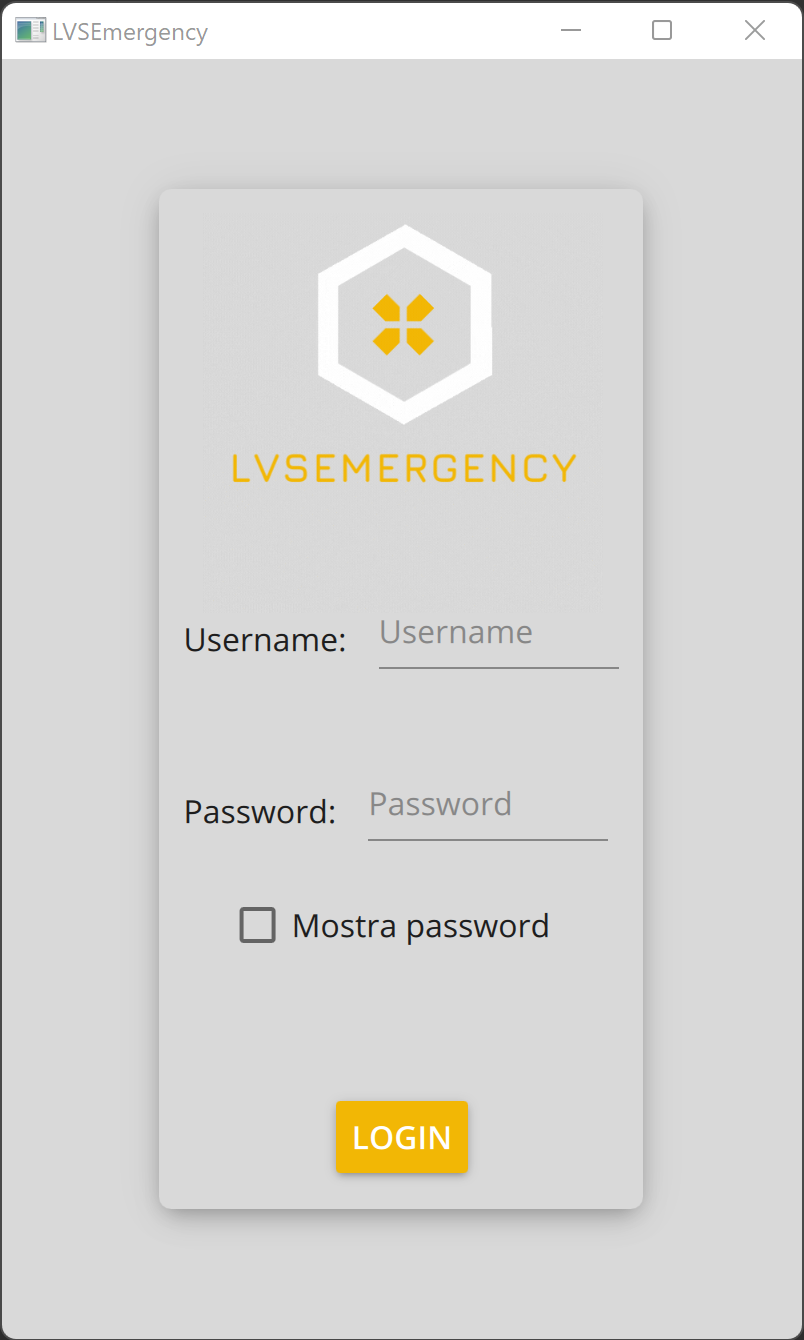
\includegraphics[width=4cm]{./Conclusione/ImageFiles/Login} }}%
	\qquad
	\subfloat[\centering Dashboard.]{{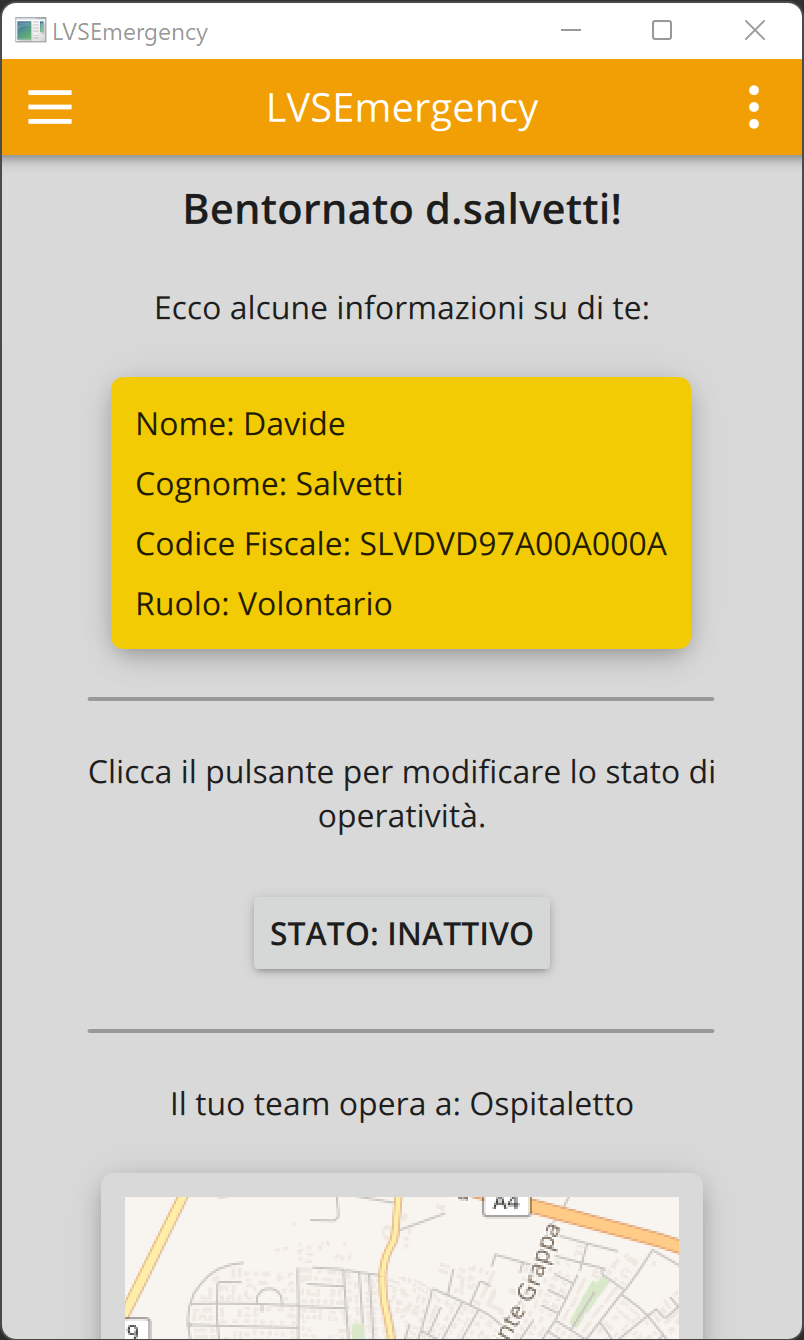
\includegraphics[width=4cm]{./Conclusione/ImageFiles/dashboard} }}%
	\qquad
	\subfloat[\centering Pannello laterale.]{{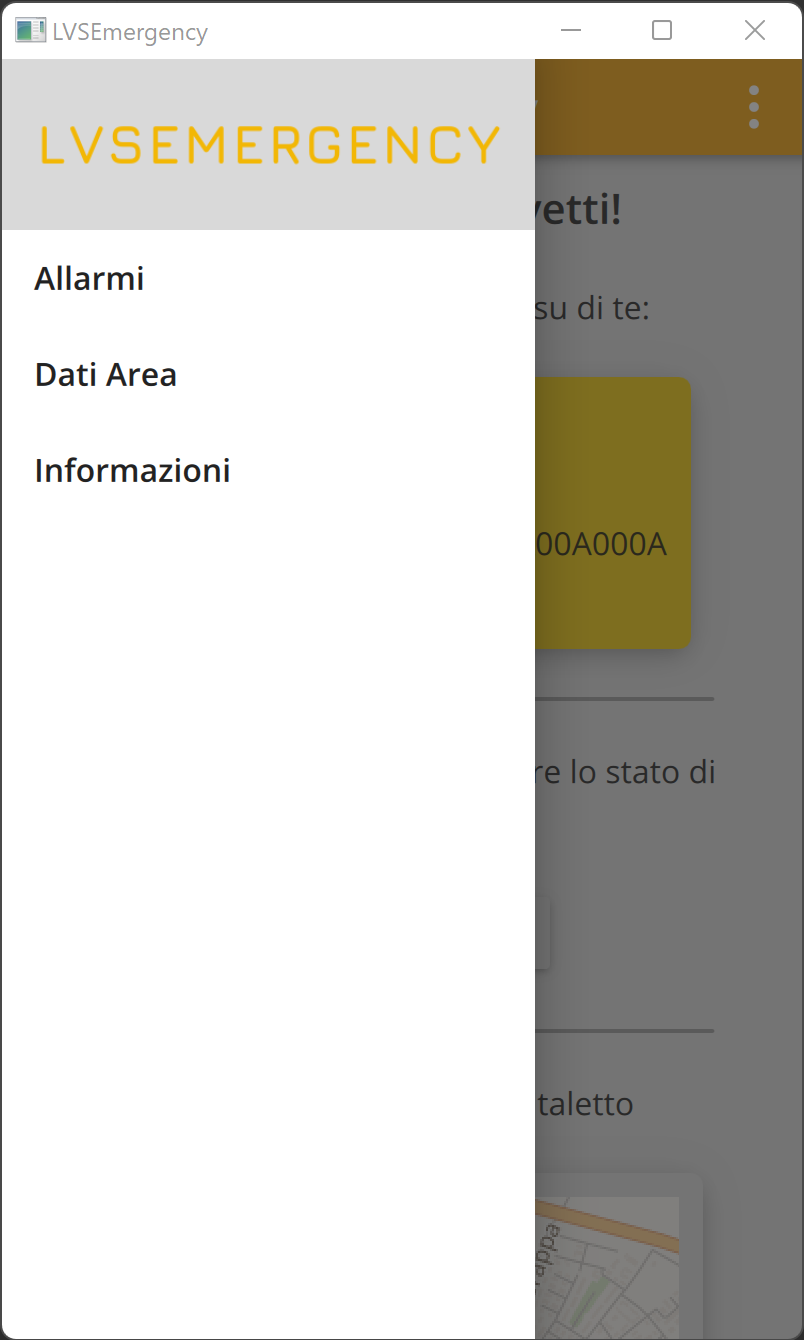
\includegraphics[width=4cm]{./Conclusione/ImageFiles/LateraleUtente} }}%
	\qquad
	\subfloat[\centering Allarmi.]{{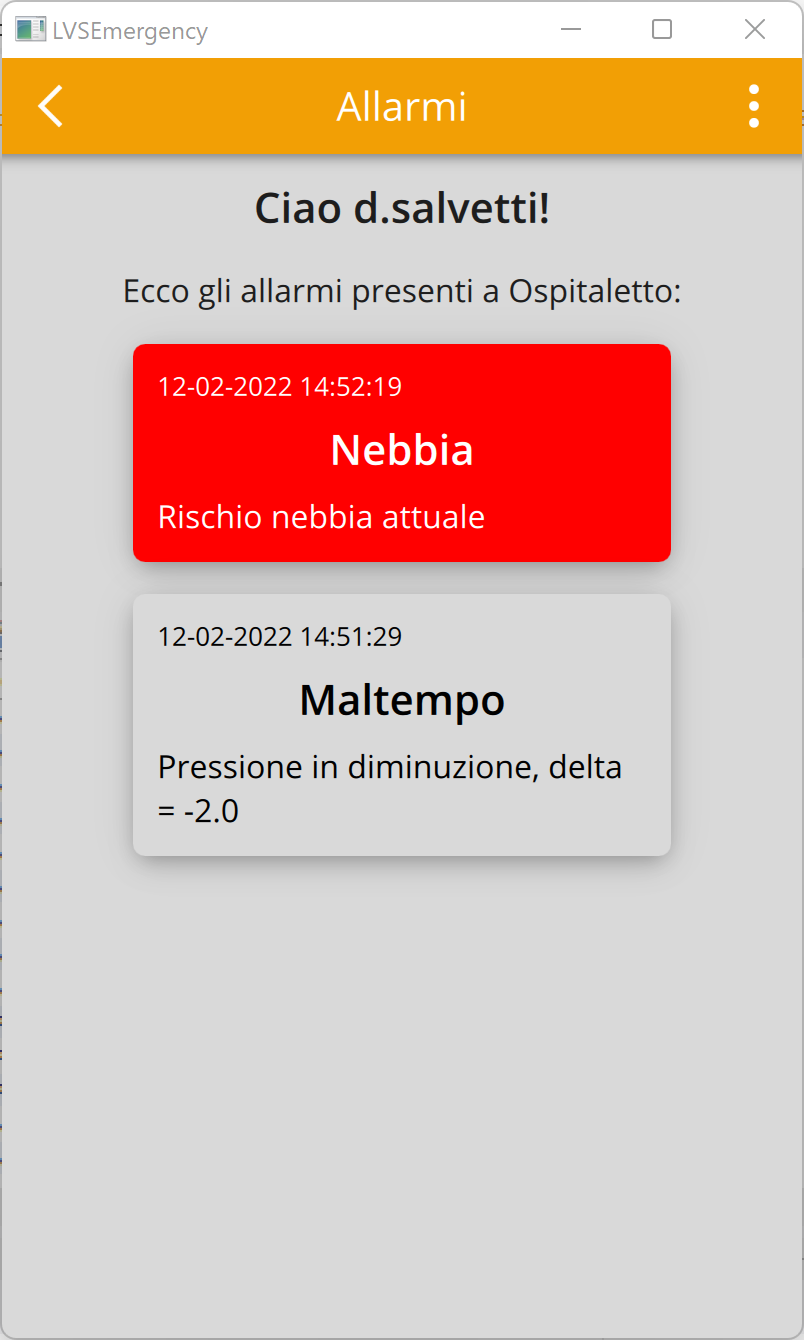
\includegraphics[width=4cm]{./Conclusione/ImageFiles/allarmi} }}%
	\qquad
	\subfloat[\centering Dati meteorologici.]{{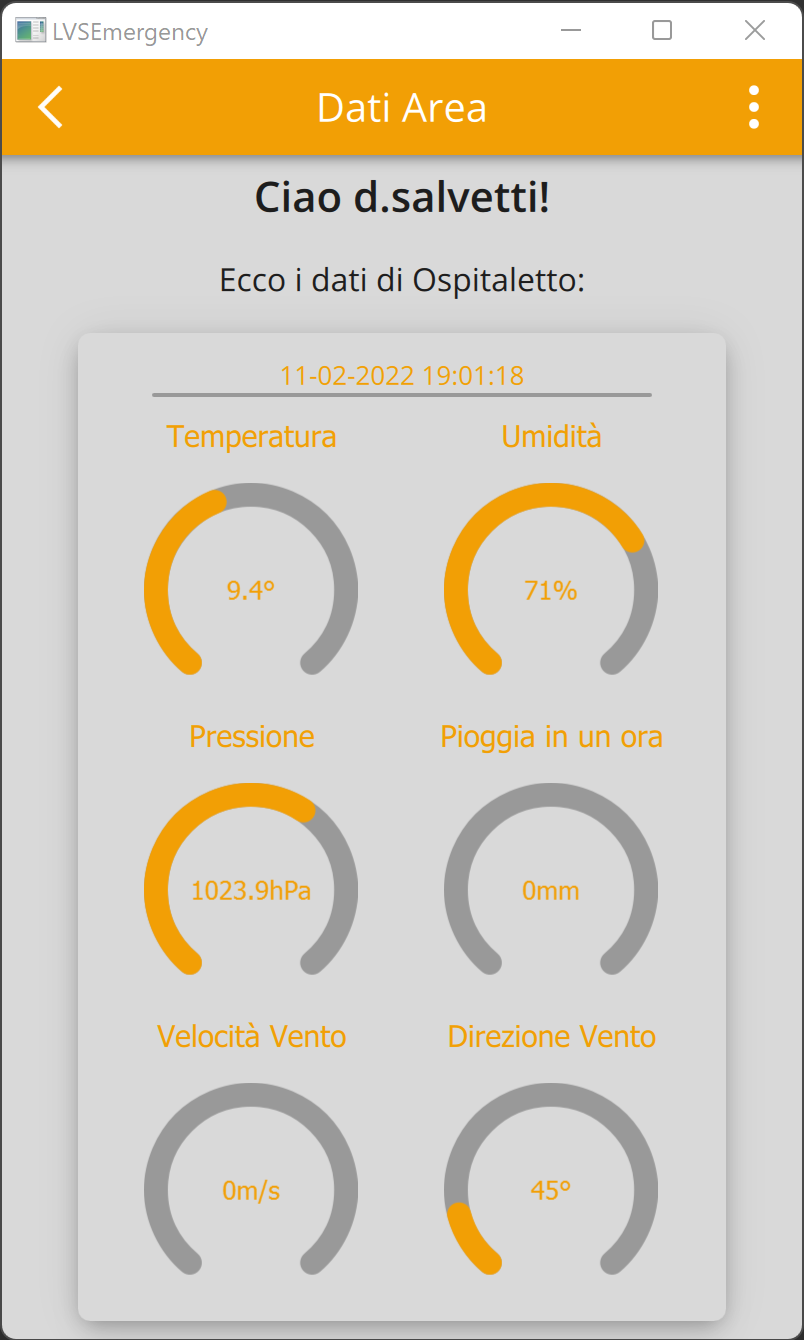
\includegraphics[width=4cm]{./Conclusione/ImageFiles/dati} }}%
	\qquad
	\subfloat[\centering Informazioni utente.]{{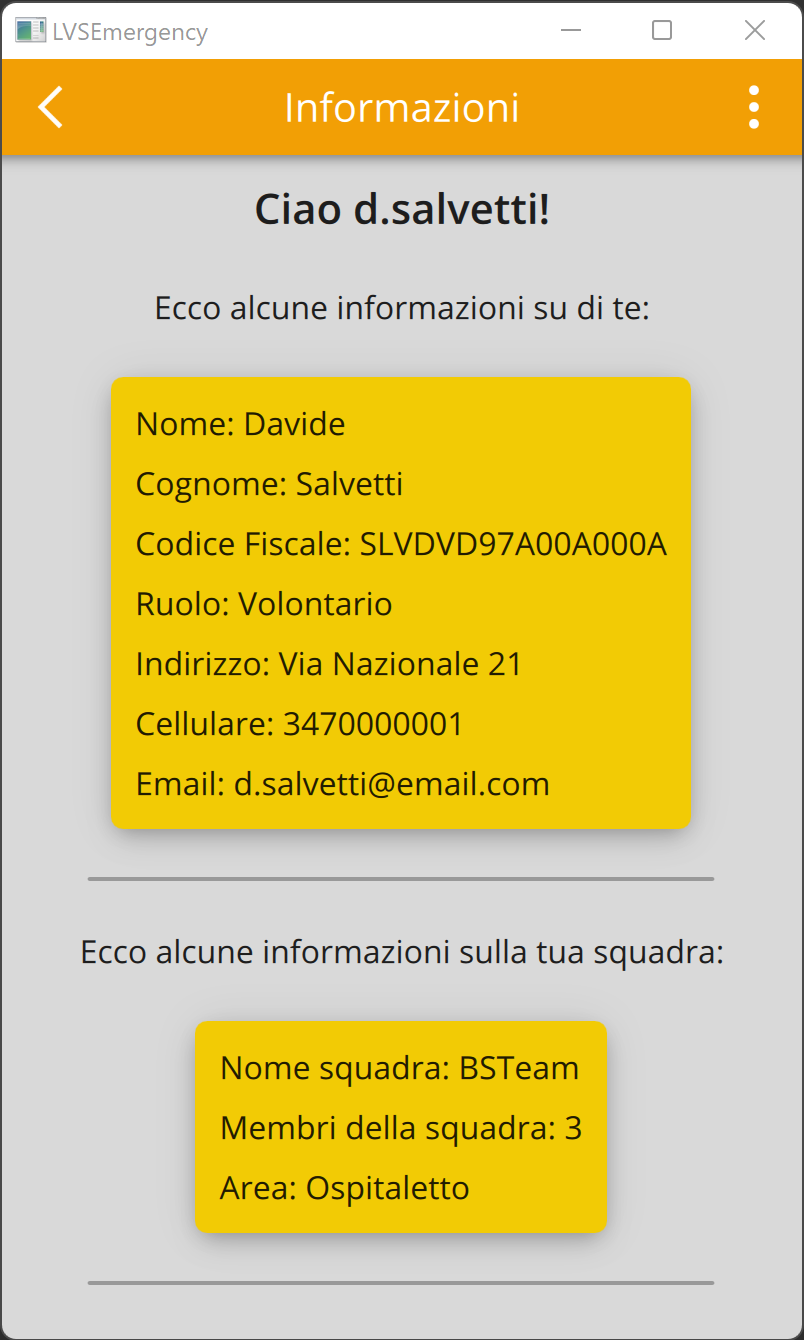
\includegraphics[width=4cm]{./Conclusione/ImageFiles/info1} }}%
	\caption{Funzionalità accessibili da volontari e caposquadra.}%
	\label{fig:qtApp}
\end{figure}


\begin{figure}[h!]
	\centering
	\subfloat[\centering Pannello laterale del coordinatore.]{{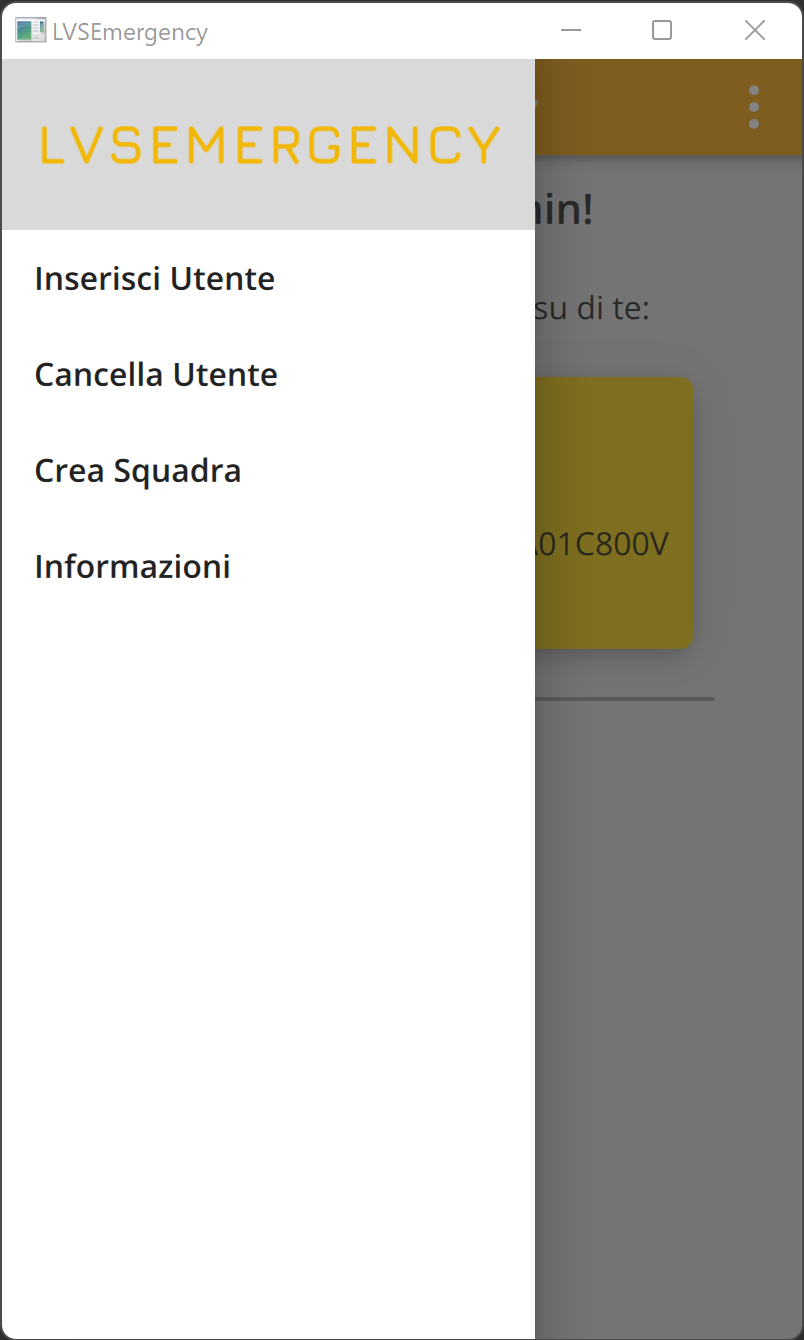
\includegraphics[width=4cm]{./Conclusione/ImageFiles/LateraleAdmin} }}%
	\qquad
	\subfloat[\centering Inserisci utente.]{{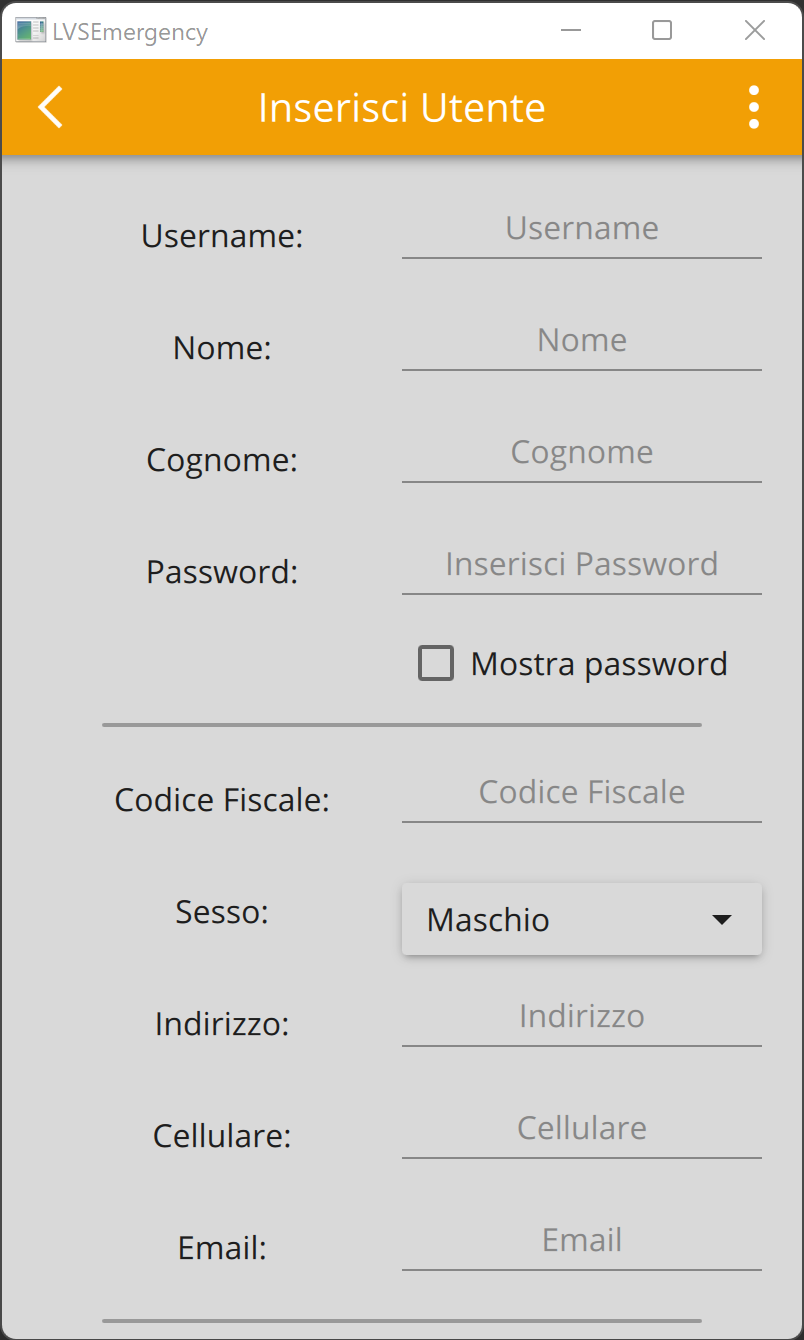
\includegraphics[width=4cm]{./Conclusione/ImageFiles/inserisciUtente} }}%
	\qquad
	\subfloat[\centering Cancella utente.]{{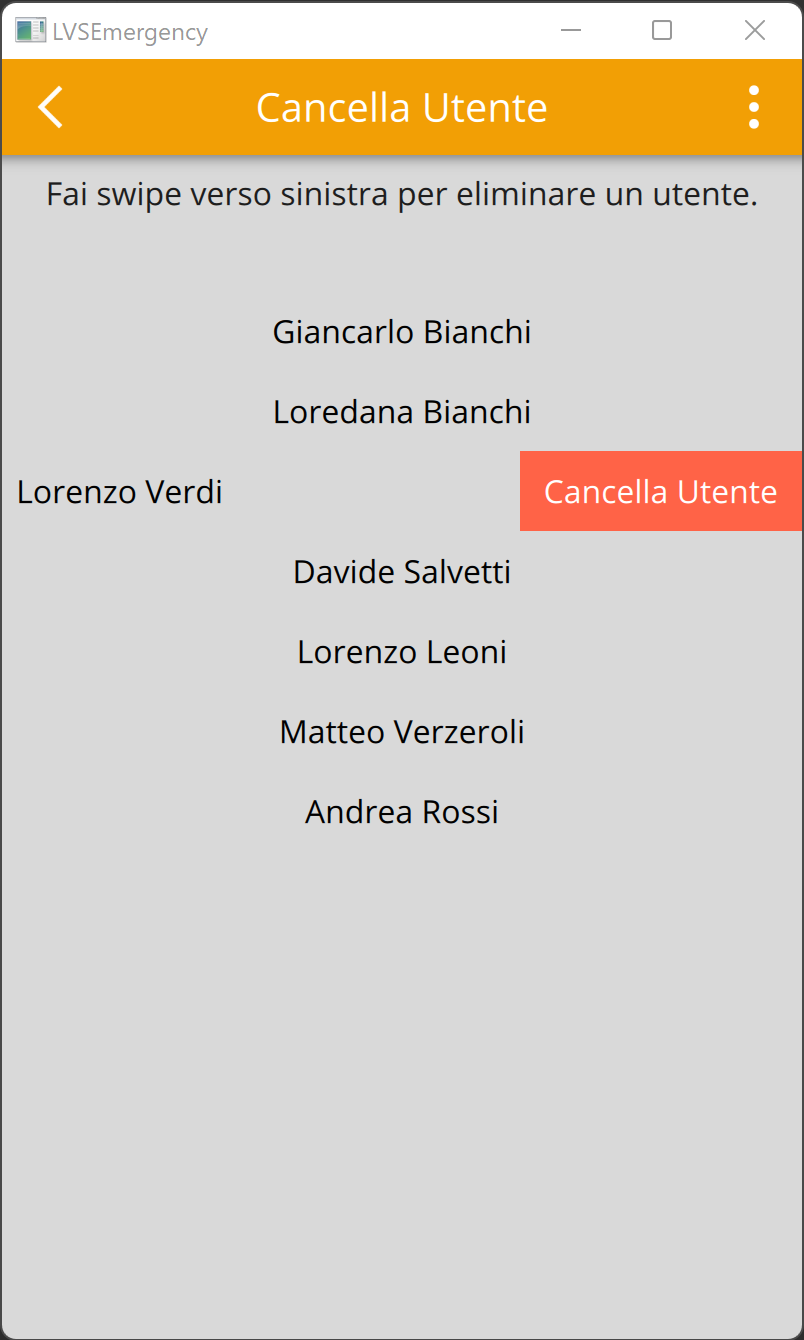
\includegraphics[width=4cm]{./Conclusione/ImageFiles/cancellaUtente} }}%
	\caption{Funzionalità accessibili dai coordinatori.}%
	\label{fig:qtApp2}
\end{figure}


\clearpage


\section{Sviluppi futuri}
Non tutti i casi d'uso definiti sono stati implementati. Di seguito è riportata una tabella riassuntiva di quali casi d'uso sono stati implementati e quali no.

\begin{center}
	\begin{tabular}{|c|c|c|}
		\hline
		\textbf{Codice} & \textbf{Caso d'uso} & \textbf{Implementato} \\ \hline
		\multicolumn{3}{|c|}{Alta Priorità} \\ \hline
		\textbf{UC1} & Login & Sì\\ \hline
		\textbf{UC2} & Logout & Sì \\ \hline
		\textbf{UC3} & Visualizzazione informazioni account & Sì \\ \hline
		\textbf{UC4} & Visualizzazione informazioni squadra & Sì \\ \hline
		\textbf{UC15} & Inserimento utente & Sì \\ \hline
		\textbf{UC16} & Cancellazione utente & Sì\\ \hline
		\textbf{UC17} & Gestione squadre (creazione) & Sì \\ \hline
		\textbf{UC18} & Visualizzazione informazioni zona & Sì \\ \hline
		\multicolumn{3}{|c|}{Media Priorità} \\ \hline
		\textbf{UC6} & Segnalazione operatività & Sì\\ \hline
		\textbf{UC7} & Visualizzazione intervento di emergenza & No \\ \hline
		\textbf{UC8} & Visualizzazione intervento programmato & No \\ \hline
		\textbf{UC9} & Inserimento informazioni intervento & No \\ \hline
		\textbf{UC11} & Gestione intervento di emergenza & No \\ \hline
		\textbf{UC12} & Gestione intervento programmato & No \\ \hline
		\textbf{UC13} & Gestione report intervento di emergenza & No \\ \hline
		\textbf{UC14} & Gestione report intervento programmato & No \\ \hline
		\textbf{UC20} & Gestione informazioni relative alla zona & No \\ \hline
		\multicolumn{3}{|c|}{Bassa Priorità} \\ \hline
		\textbf{UC5} & Gestione reperibilità & No\\ \hline
		\textbf{UC10} & Visualizzazione posizione real-time & No\\ \hline
		\textbf{UC19} & Notifiche allarmi zona & No\\ \hline
	\end{tabular}
\end{center}
 